% =====================================================================
% CHAPITRE 1 - INTRODUCTION GENERALE
% =====================================================================
% Packages recommandes a inclure dans le preambule de votre document
% principal (si ce n'est deja fait) :
%
% \usepackage[utf8]{inputenc}
% \usepackage[T1]{fontenc}
% \usepackage[french]{babel}
% \usepackage{graphicx}
% \usepackage{booktabs}
% \usepackage{array}
% \usepackage{enumitem}
% \usepackage{hyperref}
% \usepackage{xcolor}
% \usepackage{tabularx}
% =====================================================================
\chapter{Introduction Générale}
\section{Introduction Générale}
\label{chap:introduction}

La transformation numérique des entreprises impose aujourd'hui des défis sans précédent en matière de gestion et d'intégration des données. Parmi ces défis, la migration de données, processus consistant à transférer de manière sécurisée et contrôlée les données d'un système source vers un système cible, constitue un enjeu stratégique majeur. C'est dans ce contexte que s'inscrit le présent Projet de Fin d'Études, réalisé au sein de l'équipe ADMP (Accenture Data Migration Platform) d'Accenture, et portant sur le développement d'une plateforme de migration de données basée sur l'intelligence artificielle pour l'amélioration et l'optimisation des processus d'intégration des données.

% =====================================================================
\section{Organisme d'accueil}
\label{sec:organisme}

% ---------------------------------------------------------------------


% ---------------------------------------------------------------------
\subsection{Présentation d'Accenture}
\label{subsec:accenture}

Accenture plc est une entreprise multinationale de services professionnels, fondée en 1989 sous le nom d'Andersen Consulting avant de devenir Accenture en 2001, et dont le siège social est situé à Dublin, en Irlande. Cotée à la Bourse de New York (NYSE : ACN), Accenture figure parmi les plus grandes entreprises mondiales de conseil et de services technologiques.
En termes de performance financière, l'exercice fiscal 2025 (clos le 31 août 2025) témoigne de la solidité et de l'envergure du groupe, comme l'illustre le Tableau~\ref{tab:accenture-fy25}.

\begin{table}[h!]
\centering

\begin{tabular}{ll}
\toprule
\textbf{Indicateur} & \textbf{Valeur (FY 2025)} \\
\midrule
Chiffre d'affaires & 69,7 milliards USD (+7\%) \\
Résultat net (GAAP) & 7,83 milliards USD \\
Nouvelles commandes (\textit{bookings}) & 80,6 milliards USD \\
Effectif mondial & $\approx$ 779 000 collaborateurs \\
Clients servis & $\approx$ 9 000 dans plus de 120 pays \\
Bureaux et opérations & 200+ villes dans 52 pays \\
\bottomrule
\end{tabular}
\caption{Indicateurs clés d'Accenture pour l'exercice fiscal 2025}
\label{tab:accenture-fy25}
\end{table}

\begin{figure}[h]
    \centering
     
\includegraphics[width=0.3\textwidth]{img/logoaccenture.png}
    \caption{Logo du groupe Accenture}
    \label{fig:logo-accenture}
\end{figure}


L'entreprise s'articule autour de plusieurs domaines d'activité complémentaires : Strategy \& Consulting, Technology, Operations, Accenture Song (ex-Interactive) et Industry X. Sa stratégie repose sur l'ambition d'être le \textit{reinvention partner of choice} de ses clients, en combinant expertise sectorielle approfondie, partenariats écosystémiques et investissements massifs dans l'innovation.

L'intelligence artificielle occupe une place centrale dans la stratégie d'Accenture. En 2023, le groupe a annoncé un investissement de \textbf{3 milliards de dollars sur trois ans} dans sa practice \textit{Data \& AI}, visant à doubler ses effectifs IA à 80 000 professionnels et à créer des accélérateurs pour 19 secteurs industriels distincts. Les résultats de cet investissement sont déjà visibles : en FY 2025, le chiffre d'affaires lié à l'IA avancée (GenAI, IA agentique, IA physique) a triplé pour atteindre \textbf{2,7 milliards USD}, avec des commandes GenAI de \textbf{5,9 milliards USD} et plus de \textbf{6 000 projets d'IA avancée} livrés au cours de l'exercice. L'effectif Data \& AI est passé de 40 000 à \textbf{77 000 professionnels}, et plus de 550 000 collaborateurs ont été formés aux fondamentaux de l'IA générative.

% ---------------------------------------------------------------------
\subsection{Accenture au Maroc}
\label{subsec:accenture-maroc}

Au Maroc, Accenture est implantée à Casablanca, au sein du parc technologique \textbf{Casanearshore} (Sidi Maarouf), Shore 10, Park 1100, Boulevard Al Qods. Sous les entités \textbf{Accenture Morocco} et \textbf{Accenture Maghreb}, la filiale marocaine fournit des prestations de services en conseil en management, en télécommunications et en technologies de l'information. Le centre de Casablanca sert de hub nearshore pour les projets européens et africains, offrant un accès à un vivier de talents qualifiés et à un environnement opérationnel compétitif.

Le site de \textbf{Rabat, Meditech} accueille également des équipes Accenture, dont l'équipe ADMP au sein de laquelle ce PFE a été réalisé. Ce positionnement géographique permet une collaboration étroite avec les équipes européennes (principalement basées en France et en Espagne) tout en bénéficiant de la proximité culturelle et linguistique avec les clients francophones.

% ---------------------------------------------------------------------
\subsection{Positionnement de l'équipe ADMP au sein d'Accenture}
\label{subsec:admp-positionnement}

L'\textbf{Accenture Data Migration Platform (ADMP)} est une capacité de migration propriétaire développée par Accenture depuis plus de \textbf{25 ans}, dédiée à l'accélération, l'automatisation et la sécurisation des projets de migration de données à grande échelle.

L'équipe ADMP se positionne au sein de la practice \textbf{Technology, Data \& AI} et constitue un centre d'expertise spécialisé dans la migration de systèmes legacy vers des plateformes modernes. Son périmètre d'intervention est mondial et couvre trois géographies : North America, APAC et EMEA.

Les chiffres clés de l'ADMP, présentés dans le Tableau~\ref{tab:admp-kpi}, illustrent sa maturité et son envergure.

\begin{table}[h!]
\centering
\caption{Indicateurs clés de la plateforme ADMP}
\label{tab:admp-kpi}
\begin{tabular}{ll}
\toprule
\textbf{Indicateur} & \textbf{Valeur} \\
\midrule
Années d'expérience & +25 ans \\
Migrations gérées & +200 projets \\
Objets métier migrés & +75 millions \\
Spécialistes techniques et fonctionnels & +55 \\
Géographies couvertes & 3 (NA, APAC, EMEA) \\
Coût de licence & Aucun \\
Réduction des coûts vs approche non industrielle & Jusqu'à 66\% \\
\bottomrule
\end{tabular}
\end{table}

L'ADMP a servi des clients majeurs dans des secteurs variés, principalement l'assurance (Generali, AXA, Chubb, QBE, MMA, Allianz, AG2R La Mondiale), les utilities (SAUR) et l'industrie (Legrand, Bureau Veritas), avec des systèmes cibles tels que Duck Creek, Guidewire, Salesforce, Vitech et SAP.

La plateforme repose sur trois piliers fondamentaux :

\begin{itemize}[leftmargin=*]
    \item \textbf{Smart Designs} : des documents structurés (Word/Excel) qui décrivent les règles de transformation, les mappings de champs, les relations entre tables et les contraintes métier. Ces documents sont lisibles par les équipes fonctionnelles tout en étant interprétables automatiquement par la plateforme pour générer les programmes de migration.
    
    \item \textbf{Cycle ETL automatisé} : à partir des Smart Designs, ADMP génère automatiquement les programmes d'extraction, transformation et chargement, sans nécessiter de développeurs ETL traditionnels.
    
    \item \textbf{Qualité et traçabilité} : la plateforme intègre des modules de validation (pre-load et post-load), des contrôles d'intégrité, des tableaux de bord de suivi et des rapports d'anomalies facilitant les itérations entre équipes techniques et fonctionnelles.
\end{itemize}

Dans le cadre de son programme d'évolution stratégique, l'équipe ADMP a initié l'intégration de l'intelligence artificielle au sein de la plateforme, articulée autour de trois axes majeurs : l'\textbf{ADMP AI Engine} (moteur d'IA pour l'automatisation de la validation, la génération de règles et les suggestions en temps réel), l'\textbf{ADMP Studio} (outil web de design remplaçant les plugins VBA) et l'amélioration des \textbf{outils de design existants} par infusion de GenAI. C'est précisément dans ce programme d'innovation que s'inscrit le présent PFE.

% ---------------------------------------------------------------------
\section{Présentation d'AFDTech}
\label{subsec:Afdtech}


Fondée en \textbf{1998} par Jérôme Picard, \textbf{AFD.Tech} est une société française de conseil et d'ingénierie qui s'est progressivement imposée comme un acteur incontournable du marché des infrastructures informatiques, des réseaux et des télécommunications. Initialement positionnée sur le conseil de haut niveau dans le domaine télécom, au point d'avoir longtemps été qualifiée de \textit{« Pure Player Télécom »}, l'entreprise a su, au fil des années, élargir son champ d'expertise pour accompagner les grandes entreprises dans l'ensemble de leur transformation digitale : ingénierie réseau, cybersécurité, cloud computing, gestion des données, automatisation et intelligence artificielle.

Avec une croissance annuelle soutenue, AFD.Tech intervient aujourd'hui sur des projets complexes auprès de clients majeurs des secteurs bancaire, assurance, énergie, transport, télécommunications et services publics. Son implantation géographique s'étend sur trois pays (France, Belgique et Maroc) et compte aujourd'hui une dizaine de bureaux répartis entre Paris, Bruxelles, Rabat, Lyon, Strasbourg, Lille, Nantes, Toulouse, Marseille et Rennes.

Le tableau \ref{tab:afdtech-info} synthétise les principales informations relatives à l'entreprise.

\begin{figure}[h]
    \makebox[\textwidth][c]{%
        $\vcenter{\hbox{
\includegraphics[height=18mm,keepaspectratio]{img/logoNoAcc.png}}}$
        \hspace{12mm}
        {\LARGE\textbf{X}}
        \hspace{12mm}
        $\vcenter{\hbox{
\includegraphics[height=26mm,keepaspectratio]{img/logoaccenture.png}}}$
    }
    \caption{Logo d'AFD.Tech Part of Accenture}
    \label{fig:logo-afdtech}
\end{figure}

\begin{table}[h]
\centering
\renewcommand{\arraystretch}{1.3}
\begin{tabular}{|l|l|}
\hline
\textbf{Attribut} & \textbf{Valeur} \\
\hline
Raison sociale & AFD.Tech Part of Accenture \\
\hline
Année de création & 1998 \\
\hline
Fondateur & Jérôme Picard \\
\hline
Siège social & Paris, France \\
\hline
Présence internationale & France, Belgique, Maroc \\
\hline
Implantation au Maroc & Depuis 2014 (Rabat) \\
\hline
Effectif global & Plus de 1 600 collaborateurs \\
\hline
Effectif au Maroc & Plus de 900 collaborateurs \\
\hline
Secteurs d'activité & Télécoms, IT, Cloud, Cybersécurité, Data, IA \\
\hline
Site web & \url{https://afd.tech} \\
\hline
\end{tabular}
\caption{Informations clés sur AFD.Tech Part of Accenture}
\label{tab:afdtech-info}
\end{table}



% ---------- 1.1.2 Le rapprochement avec Accenture ----------
\subsection{Le rapprochement avec Accenture}

L'année 2022 marque un tournant majeur dans l'histoire de l'entreprise. Le \textbf{1\textsuperscript{er} avril 2022}, AFD.Tech rejoint officiellement le groupe \textbf{Accenture}, leader mondial des services aux entreprises et administrations, à l'issue d'une opération de rachat à 100\,\% du capital annoncée le 15 décembre 2021. Cette acquisition, motivée par la volonté d'Accenture de renforcer ses capacités en services réseaux autour des technologies 5G, fibre et \textit{cloud-first networks}, s'est traduite par l'intégration de plus de 1\,600 professionnels hautement qualifiés au sein du groupe.

Désormais désignée sous la dénomination \textbf{AFD.Tech Part of Accenture}, l'entreprise a conservé sa culture d'expertise technique tout en bénéficiant de la dimension internationale, des moyens et de l'écosystème d'innovation d'Accenture. Cette intégration stratégique a permis à AFD.Tech d'élargir significativement son périmètre commercial : alors que ses clients étaient historiquement basés en France (à hauteur de 90\,\%) et en Belgique, l'entreprise travaille aujourd'hui également avec des clients au Benelux, en Italie et au Royaume-Uni.

% ---------- 1.1.3 AFD.Tech au Maroc ----------

\subsection{AFD.Tech au Maroc : MEDITECH et MEDxp}

L'implantation marocaine d'AFD.Tech, démarrée en \textbf{2014} avec une équipe de quelques dizaines d'ingénieurs, a connu une croissance exponentielle pour devenir aujourd'hui l'un des piliers du développement nearshore du groupe. Cette dynamique s'est concrétisée par la création successive de deux centres d'excellence dédiés aux nouvelles technologies à Rabat.

\paragraph{MEDITECH.} Inauguré en 2021, MEDITECH a été le premier centre d'innovation d'AFD.Tech au Maroc. Construit sur \textbf{2\,000~m\textsuperscript{2}} et accueillant aujourd'hui \textbf{plus de 300 ingénieurs}, il a été conçu dès l'origine comme un lieu d'excellence technologique, ouvert et collaboratif, capable d'incarner l'identité innovante du groupe. Il a posé les fondations de la stratégie d'expansion marocaine et constitue toujours le c\oe ur opérationnel des activités locales.

\paragraph{MEDxp.} Ouvert en avril 2023, MEDxp prolonge cette dynamique avec une vocation encore plus orientée vers les technologies de pointe. Ce second pôle, également de 2\,000~m\textsuperscript{2}, est dédié aux nouvelles technologies et accueille plus de 300 ingénieurs experts en \textbf{5G, intelligence artificielle et data science}. Au-delà de sa dimension technique, MEDxp se veut un espace de culture et de partage, centré sur l'expérience offerte aux candidats et aux collaborateurs.

\begin{figure}[h]
    \centering
     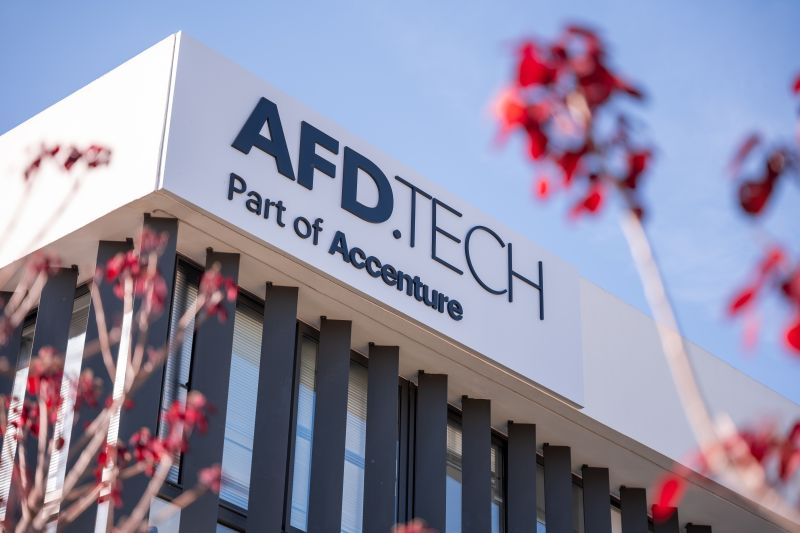
\includegraphics[width=0.8\textwidth]{img/image-afdtech.PNG}
    \caption{Le centre d'excellence MEDITECH à Rabat}
    \label{fig:meditech}
\end{figure}

L'équipe marocaine compte aujourd'hui \textbf{plus de 900 experts} et joue un rôle crucial dans l'évolution du groupe. Elle est dirigée par \textbf{Amine El Rhayour}, \textit{Director of the Service Delivery Center Morocco}, dont le parcours d'ingénieur incarne la trajectoire d'excellence technique portée par l'entreprise au Maroc. L'organisation interne s'articule autour de plusieurs pôles stratégiques, comme illustré par la figure \ref{fig:organigramme}.

\begin{figure}[h]
    \centering
    % \includegraphics[width=\textwidth]{img/organigramme_afdtech.png}
    \caption{Organigramme du centre AFD.Tech Maroc}
    \label{fig:organigramme}
\end{figure}

L'expertise déployée à Rabat couvre un périmètre étendu : ingénierie réseau et télécoms, transformation digitale, cloud computing, intelligence artificielle, data science et migration de données. C'est précisément dans ce dernier domaine, au sein de l'équipe ADMP, que s'inscrit le présent stage de fin d'études.


% =====================================================================
\section{Contexte académique}
\label{sec:contexte-academique}

% ---------------------------------------------------------------------
\subsection{Présentation de l'Université Internationale de Rabat}
\label{subsec:uir}

L'\textbf{Université Internationale de Rabat (UIR)} est une université privée d'excellence fondée en 2010, située sur le campus Technopolis à Rabat-Salé. Reconnue par l'État marocain, l'UIR propose des formations innovantes dans les domaines de l'ingénierie, de l'architecture, du management (Rabat Business School), du droit, des sciences politiques, des énergies renouvelables et des sciences de la santé.

Partenaire de grandes universités françaises et européennes, notamment l'Université de Nantes, l'UIR offre des doubles diplômes et une forte ouverture internationale à ses étudiants. L'université s'est distinguée récemment par un palmarès historique au Salon International des Inventions de Genève (4 médailles et un prix spécial) et par l'intégration de Rabat Business School dans le classement QS Executive MBA 2026.

\begin{figure}[h]
    \centering
     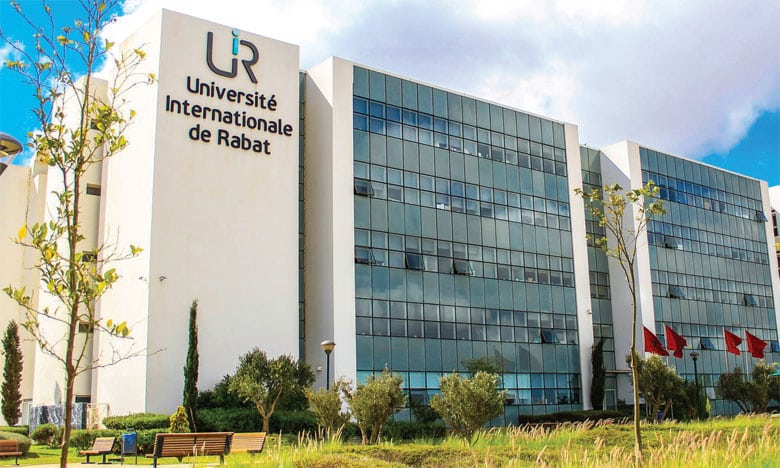
\includegraphics[width=0.7\textwidth]{img/imageuir.jpg}
    \caption{L'Université Internationale de Rabat}
    \label{fig:uir}
\end{figure}


% ---------------------------------------------------------------------
\subsection{L'École Supérieure d'Informatique et du Numérique (ESIN)}
\label{subsec:esin}

Le présent PFE est réalisé dans le cadre de la formation d'\textbf{ingénieur en informatique} dispensée par l'\textbf{École Supérieure d'Informatique et du Numérique (ESIN)}, composante de l'UIR. L'ESIN a pour mission de former des informaticiens hautement qualifiés et de mener des activités de recherche accompagnant le développement technologique et économique du Maroc.

La formation s'étend sur cinq ans : deux années de cycle préparatoire intégré, suivies de trois années de cycle ingénieur. La première année du cycle ingénieur constitue un tronc commun, et la deuxième année offre un choix de spécialisation entre : \textbf{Big Data}, \textbf{Ingénierie des systèmes d'information}, \textbf{Sécurité des systèmes d'information} et \textbf{Cloud Computing \& Virtualisation}.

Les objectifs pédagogiques du programme (PEO) visent à former des ingénieurs capables d'appliquer les principes de l'informatique dans un cadre professionnel, de déployer des fondements interdisciplinaires, et de résoudre de manière créative des problèmes au sein d'équipes pluridisciplinaires.

L'ESIN est née d'un partenariat académique entre l'UIR et l'Université de Nantes, et bénéficie de partenariats industriels avec des entreprises de premier plan, assurant ainsi une pédagogie axée sur l'insertion professionnelle et le rapprochement avec le monde socio-économique.


% =====================================================================
\section{Cadrage du projet de stage}
\label{sec:cadrage}

% ---------------------------------------------------------------------
\subsection{Sujet et périmètre de la mission}
\label{subsec:sujet}

Le sujet de ce PFE s'intitule : \og~\textbf{Développement d'une plateforme de migration de données basée sur l'IA pour l'amélioration et l'optimisation des processus d'intégration des données}~\fg{}.

Il s'inscrit dans le programme d'évolution d'ADMP visant à intégrer l'intelligence artificielle au cœur de la plateforme. Les objectifs stratégiques de cette intégration sont triples :

\begin{itemize}[leftmargin=*]
    \item \textbf{Rester un différenciateur réel} en matière de migration grâce à un moteur IA dédié (ADMP AI Engine).
    \item \textbf{Optimiser et accélérer} le temps nécessaire à la rédaction des spécifications de migration, et automatiser l'analyse des audits de données.
    \item \textbf{Créer un véritable assistant intelligent} pour les spécificateurs, réduisant la charge globale de travail.
\end{itemize}

Le périmètre de la mission couvre principalement la \textbf{génération du bundle Databricks}, un module central de la nouvelle architecture ADMP, dont les détails techniques seront présentés dans les chapitres~5 et~6. Ce module vise à automatiser la création des artefacts de migration en s'appuyant sur des technologies de traitement distribué (Apache Spark / Databricks) et d'intelligence artificielle générative.

% ---------------------------------------------------------------------
\subsection{Objectifs opérationnels et livrables attendus}
\label{subsec:objectifs}

Les objectifs opérationnels du PFE se déclinent comme suit :

\begin{itemize}[leftmargin=*]
    \item \textbf{Comprendre et maîtriser} la méthodologie ADMP et ses livrables (SDS, IDS, TDS, DS, RC, DP, TT, MS) à travers la formation Core ADMP Design School (CIDS).
    \item \textbf{Contribuer opérationnellement} aux projets de migration en cours, notamment en matière d'analyse de données, de validation de tickets et de rédaction de spécifications.
    \item \textbf{Concevoir et implémenter} le module de génération du bundle Databricks dans le cadre de l'évolution IA de la plateforme.
    \item \textbf{Tester et valider} la solution développée sur des cas réels de migration.
    \item \textbf{Documenter} l'ensemble du travail réalisé dans le présent rapport de PFE.
\end{itemize}

Ce travail s'inscrit dans la continuité des contributions précédentes de l'équipe : le PFE de Elharrioui Aymen portant sur la conception d'un agent intelligent basé sur RAG et l'architecture AppSync/GraphQL, et le PFE de Majbar Nizar portant sur le fine-tuning d'un LLM (Mistral 7B avec LoRA) pour la génération de règles de transformation.

% ---------------------------------------------------------------------
\subsection{Planning prévisionnel}
\label{subsec:planning}

Le stage se déroule sur une période de six mois, organisée en phases progressives, comme le résume le Tableau~\ref{tab:planning}.

\begin{table}[h!]
\centering
\caption{Planning prévisionnel du stage}
\label{tab:planning}
\begin{tabularx}{\textwidth}{l l X}
\toprule
\textbf{Phase} & \textbf{Période} & \textbf{Activités principales} \\
\midrule
Intégration \& Formation & Mois 1--2 & Onboarding, CIDS (2 semaines), découverte des outils et de la méthodologie ADMP \\
\addlinespace
Contribution opérationnelle & Mois 2--4 & Participation aux projets de migration, analyse de données, gestion de tickets, validation \\
\addlinespace
Conception \& Développement & Mois 3--5 & Conception et implémentation du module de génération du bundle Databricks \\
\addlinespace
Tests \& Validation & Mois 5--6 & Tests, évaluation, documentation, rédaction du rapport \\
\bottomrule
\end{tabularx}
\end{table}

\textit{Un diagramme de Gantt détaillé est présenté en annexe.}

% =====================================================================
\section{Organisation du rapport}
\label{sec:organisation}

Le présent rapport est structuré selon une logique narrative séquentielle, guidant le lecteur depuis la compréhension du problème jusqu'à la validation de la solution proposée :

\begin{itemize}[leftmargin=*]
    \item \textbf{Chapitre 2, Contexte et Problématique} : présente de manière générique les enjeux et défis de la migration de données, indépendamment de tout projet client, et formule la problématique de recherche.
    
    \item \textbf{Chapitre 3, État de l'Art} : explore les fondements théoriques de la migration, les solutions existantes sur le marché (outils ETL, services cloud), la plateforme ADMP dans son état actuel, les avancées de l'IA dans l'intégration de données, et identifie les limites et opportunités qui positionnent notre contribution.
    
    \item \textbf{Chapitre 4, Cadre Méthodologique et Gestion de Projet} : décrit l'organisation agile du travail, le cycle de vie des tickets, les processus de validation des données et les pratiques collaboratives de l'équipe.
    
    \item \textbf{Chapitre 5, Conception et Architecture de la Solution} : présente exclusivement les éléments nouveaux de notre contribution, l'architecture IA cible et le module de génération du bundle Databricks, en s'appuyant sur la description de l'existant fournie au chapitre~3.
    
    \item \textbf{Chapitre 6, Implémentation} : détaille la réalisation technique des modules, l'environnement de développement, et les difficultés rencontrées avec leurs solutions.
    
    \item \textbf{Chapitre 7, Résultats et Évaluation} : présente le protocole de test, les résultats obtenus et une discussion critique de la solution.
    
    \item \textbf{Chapitre 8, Conclusion et Perspectives} : synthétise les contributions, les compétences acquises et les pistes d'évolution futures.
\end{itemize}